% ============================================================
% Module 06: NVIDIA Ecosystem
% Custom Navasena Dark Beamer Theme
% Compiler: xelatex
% ============================================================
\documentclass[aspectratio=169,t]{beamer}

% ---- Fonts (xelatex) ----------------------------------------
\usepackage{fontspec}
\usepackage[sfdefault]{FiraSans}

% ---- Core packages ------------------------------------------
\usepackage{graphicx}
\usepackage{tikz}
\usetikzlibrary{positioning, shapes.geometric, arrows.meta, calc}
\usepackage{pgfplots}
\pgfplotsset{compat=1.18}
\usepackage{amsmath}
\usepackage{booktabs}
\usepackage{colortbl}
\usepackage{xcolor}
\usepackage{listings}

% ============================================================
% COLOR PALETTE (Navasena dark theme)
% ============================================================
\definecolor{nvbg}{HTML}{1A1A2E}
\definecolor{nvdark}{HTML}{1A1A2E}
\definecolor{nvcard}{HTML}{2D2D44}
\definecolor{nvgreen}{HTML}{76B900}
\definecolor{nvlightgreen}{HTML}{A3D944}
\definecolor{nvwhite}{HTML}{FFFFFF}
\definecolor{nvgray}{HTML}{AAAACC}
\definecolor{nvdarkcard}{HTML}{23233A}
\definecolor{nvred}{HTML}{EF5350}
\definecolor{nvorange}{HTML}{FF6F00}
\definecolor{nvblue}{HTML}{42A5F5}

% ============================================================
% LISTINGS STYLE
% ============================================================
\lstset{
  backgroundcolor=\color{nvcard},
  basicstyle=\ttfamily\small\color{nvwhite},
  keywordstyle=\color{nvgreen}\bfseries,
  stringstyle=\color{nvlightgreen},
  commentstyle=\color{nvgray}\itshape,
  numberstyle=\tiny\color{nvgray},
  numbers=left,
  numbersep=6pt,
  frame=none,
  breaklines=true,
  showstringspaces=false,
  tabsize=2,
  xleftmargin=8pt,
  xrightmargin=4pt,
}

% ============================================================
% BEAMER THEME — NAVASENA DARK
% ============================================================
\usetheme{default}
\usecolortheme{default}

\setbeamercolor{background canvas}{bg=nvbg}
\setbeamercolor{normal text}{fg=nvwhite}
\setbeamercolor{frametitle}{fg=nvwhite, bg=nvbg}
\setbeamercolor{framesubtitle}{fg=nvgray, bg=nvbg}
\setbeamercolor{title}{fg=nvgreen}
\setbeamercolor{author}{fg=nvgray}
\setbeamercolor{date}{fg=nvgray}
\setbeamercolor{item}{fg=nvgreen}
\setbeamercolor{subitem}{fg=nvlightgreen}
\setbeamercolor{subsubitem}{fg=nvgray}
\setbeamercolor{block title}{fg=nvwhite, bg=nvcard}
\setbeamercolor{block body}{fg=nvwhite, bg=nvcard}

\setbeamertemplate{footline}{%
  \hbox{%
    \begin{beamercolorbox}[wd=\paperwidth,ht=2.5ex,dp=1ex,leftskip=2em]{author in head/foot}%
      \color{nvgray}\small\textbf{NVIDIA Ecosystem} \hfill \insertframenumber\,/\,\inserttotalframenumber
    \end{beamercolorbox}%
  }%
}
\setbeamertemplate{navigation symbols}{}

% ============================================================
% CUSTOM COMMANDS
% ============================================================
\newcommand{\acttitle}[3]{%
  \begin{frame}[plain]
    \vspace{1.5cm}
    \begin{center}
      {\color{nvgreen}\Huge\bfseries Act #1}\\[1.2em]
      {\color{nvwhite}\Huge #2}\\[0.8em]
      {\color{nvgray}\Large #3}
    \end{center}
  \end{frame}%
}

\title{NVIDIA Ecosystem}
\subtitle{Navasena Gen-ML Course}
\author{Navasena AI}
\date{}

% ============================================================
\begin{document}

% Slide 1 — Title
\begin{frame}[plain]
  \vspace{1.0cm}
  \begin{center}
    {\color{nvgreen}\Huge\bfseries Module 06}\\[1.0em]
    {\color{nvwhite}\Huge\bfseries NVIDIA Ecosystem}\\[0.6em]
    {\color{nvgray}\Large GPU, NeMo, dan RAG yang dipercepat}\\[1.6em]

    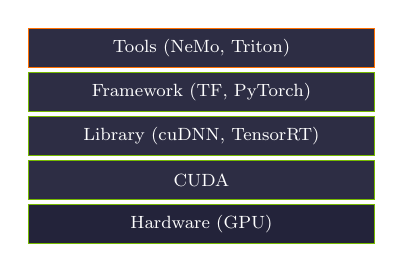
\begin{tikzpicture}[scale=0.8, every node/.style={transform shape},
        lay/.style={draw=nvgreen, fill=nvcard, text=white, font=\footnotesize, minimum width=5.5cm, minimum height=0.62cm}]
      \node[lay, fill=nvdarkcard] (h) at (0,0) {Hardware (GPU)};
      \node[lay] (c) at (0,0.7) {CUDA};
      \node[lay] (l) at (0,1.4) {Library (cuDNN, TensorRT)};
      \node[lay] (f) at (0,2.1) {Framework (TF, PyTorch)};
      \node[lay, draw=nvorange] (t) at (0,2.8) {Tools (NeMo, Triton)};
    \end{tikzpicture}

    \vspace{0.7em}
    {\color{nvgray}\small Navasena AI \quad $\cdot$ \quad 2026}
  \end{center}
\end{frame}

% ── Act 1: GPU, CUDA & Optimasi ───────────────────────────
\acttitle{1}{GPU, CUDA \& Optimasi}{Fondasi hardware \& software NVIDIA}

% Slide 2 — Stack NVIDIA
\begin{frame}{Stack NVIDIA: Dari Chip ke Tools}
  \framesubtitle{Lapisan-lapisan yang membuat AI berjalan cepat}
  \begin{columns}[T]
    \begin{column}{0.52\textwidth}
      \begin{itemize}
        \footnotesize
        \item \textbf{Hardware} $=$ GPU (T4/A100/H100)
        \item \textbf{CUDA} $=$ jembatan agar GPU bisa untuk komputasi umum
        \item \textbf{Library} $=$ cuDNN, cuBLAS, TensorRT (rutin matematika siap pakai)
        \item \textbf{Framework $+$ Tools} $=$ TF/PyTorch $+$ NeMo/Triton (tempat kita menulis kode)
      \end{itemize}
    \end{column}
    \begin{column}{0.46\textwidth}
      \begin{center}
        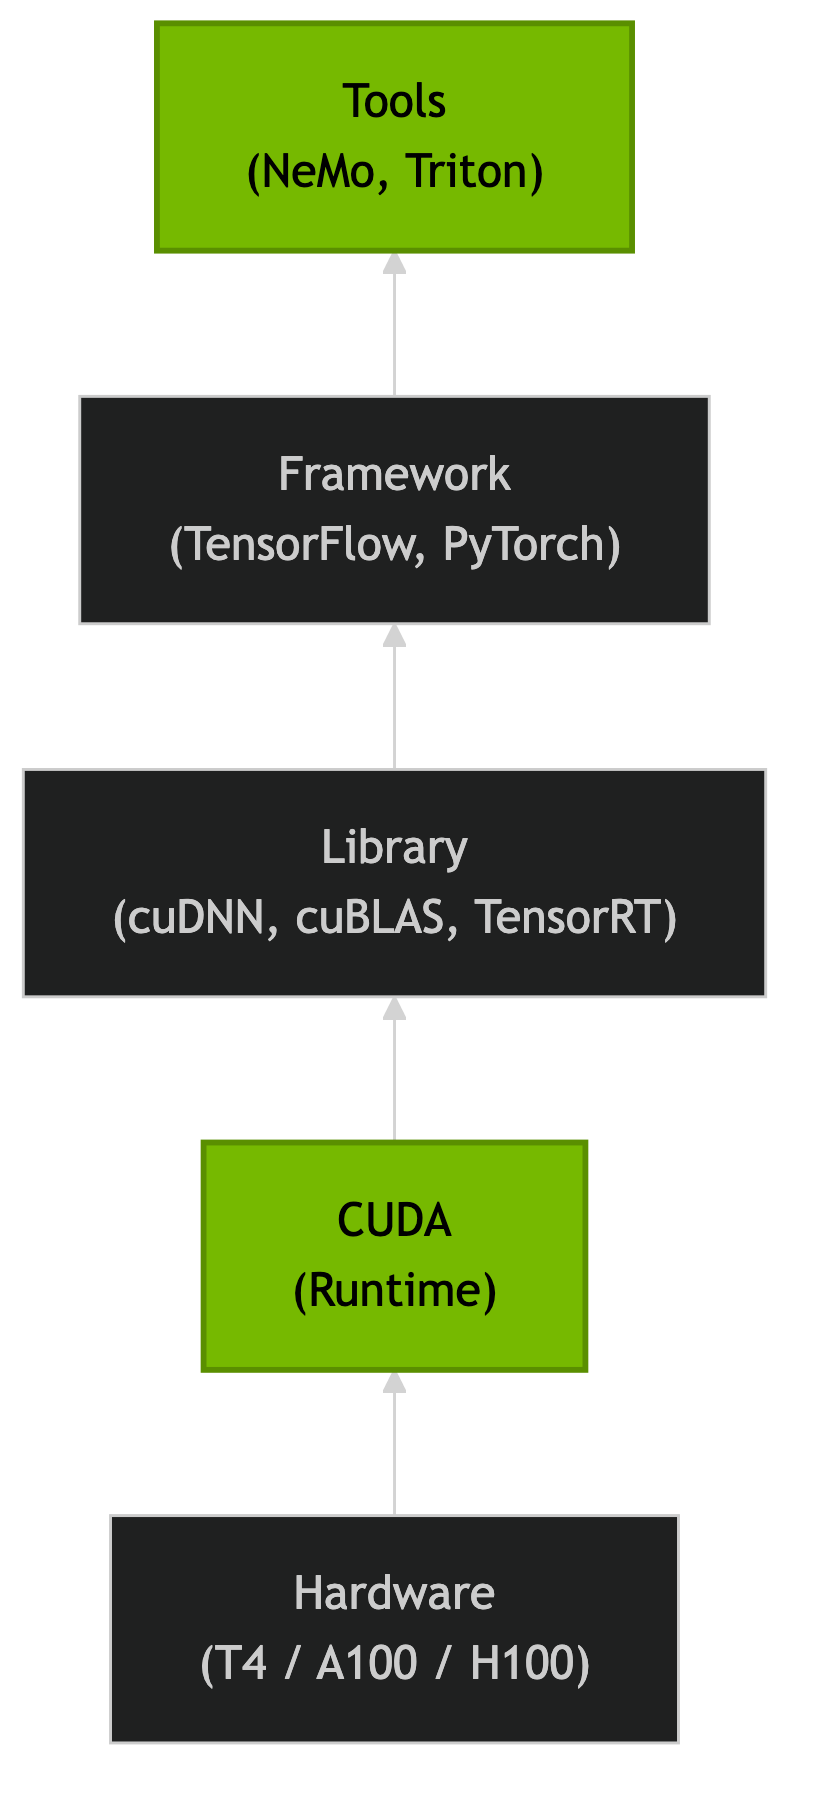
\includegraphics[height=0.54\textheight]{figures/nvidia_stack.png}
      \end{center}
    \end{column}
  \end{columns}
  \vspace{0.2em}
  \begin{center}\textcolor{nvlightgreen}{\small Tiap lapisan berdiri di atas lapisan bawahnya: kita menulis di Framework, GPU yang bekerja keras.}\end{center}
\end{frame}

% Slide 3 — Kenapa GPU (recap)
\begin{frame}{Kenapa GPU? (Recap Module 02)}
  \framesubtitle{Ribuan core paralel untuk operasi matriks}
  \begin{itemize}
    \item \textbf{CPU}: sedikit core, sangat pintar, kerja berurutan
    \item \textbf{GPU}: ribuan core sederhana, kerja \textbf{paralel} (serentak)
    \item \textbf{Deep learning} $=$ tumpukan \textbf{matrix operations} (perkalian matriks)
    \item Perkalian matriks dipecah jadi ribuan operasi kecil $\to$ pas untuk GPU
  \end{itemize}
  \vspace{0.5em}
  \begin{beamercolorbox}[rounded=true,shadow=false,sep=6pt]{block body}
    \small\color{white}
    Lihat \textbf{Module 02} untuk dasar arsitektur GPU. Catatan: notebook ini hanya mengukur waktu di GPU --- perbandingan vs CPU adalah pengetahuan umum, bukan benchmark di sini.
  \end{beamercolorbox}
\end{frame}

% Slide 4 — Benchmark phi-2
\begin{frame}[fragile]{Benchmark Model: microsoft/phi-2}
  \framesubtitle{Mengukur kecepatan inference di GPU}
  \begin{columns}[T]
    \begin{column}{0.46\textwidth}
      \begin{itemize}
        \footnotesize
        \item Memuat \textbf{microsoft/phi-2} ($\sim$2.7B parameter)
        \item \texttt{torch\_dtype=float16} (\textbf{FP16}) $\to$ hemat memori GPU
        \item \texttt{device\_map="auto"} $\to$ taruh di GPU otomatis
        \item \textbf{Warmup} 1x, lalu \texttt{generate()} 5x, dirata-rata
      \end{itemize}
    \end{column}
    \begin{column}{0.52\textwidth}
      \begin{lstlisting}[language=Python, basicstyle=\ttfamily\scriptsize\color{nvwhite}]
model = AutoModelForCausalLM.from_pretrained(
    "microsoft/phi-2",
    torch_dtype=torch.float16,  # FP16
    device_map="auto")          # ke GPU
      \end{lstlisting}
    \end{column}
  \end{columns}
  \vspace{0.2em}
  \begin{center}\textcolor{nvlightgreen}{\small Pola load model NVIDIA: \textbf{FP16} $+$ \texttt{device\_map="auto"}. Benchmark $=$ rata-rata waktu generate di GPU (tanpa baseline CPU).}\end{center}
\end{frame}

% Slide 5 — Half Precision
\begin{frame}{Half Precision: FP16 vs FP32}
  \framesubtitle{Angka 16-bit untuk hemat memori dan lebih cepat}
  \begin{columns}[T]
    \begin{column}{0.5\textwidth}
      \begin{itemize}
        \footnotesize
        \item \textbf{Mixed precision} (campur FP32+FP16): konsep umum pelatihan model
        \item \textbf{Tensor Cores}: unit GPU NVIDIA super cepat untuk FP16
        \item Notebook ini memuat phi-2 dalam \textbf{FP16 penuh} (\texttt{torch.float16}), \emph{bukan} mixed precision (tanpa AMP/autocast)
      \end{itemize}
    \end{column}
    \begin{column}{0.48\textwidth}
      \begin{center}
      \renewcommand{\arraystretch}{1.35}
      {\footnotesize
      \setlength{\tabcolsep}{4pt}
      \begin{tabular}{@{}p{0.18\linewidth}p{0.18\linewidth}p{0.54\linewidth}@{}}
        \toprule
        \rowcolor{nvcard!50}
        \textbf{Tipe} & \textbf{Bit} & \textbf{Sifat} \\
        \midrule
        FP32 & 32-bit & Presisi penuh, boros memori \\
        FP16 & 16-bit & Hemat memori $\sim$50\%, cepat di Tensor Cores \\
        \bottomrule
      \end{tabular}%
      }
      \end{center}
    \end{column}
  \end{columns}
  \vspace{0.3em}
  \begin{center}\textcolor{nvlightgreen}{\small Yang dipakai notebook: half precision (FP16 penuh). Mixed precision (AMP) dibahas di Module 02, tidak didemokan di sini.}\end{center}
\end{frame}

% Slide 6 — TensorRT
\begin{frame}{TensorRT: Optimasi Inference}
  \framesubtitle{Membuat model berjalan jauh lebih cepat saat dipakai}
  \begin{columns}[T]
    \begin{column}{0.5\textwidth}
      \begin{itemize}
        \footnotesize
        \item \textbf{TensorRT}: alat NVIDIA mempercepat \textbf{inference} (saat dipakai)
        \item \textbf{Layer fusion} $+$ \textbf{kernel auto-tuning}
        \item \textbf{Precision calibration}: turun ke FP16/INT8, akurasi terjaga
        \item \textbf{TF-TRT}: tipikal 2--5$\times$ lebih cepat (angka NVIDIA)
      \end{itemize}
    \end{column}
    \begin{column}{0.48\textwidth}
      \begin{center}
      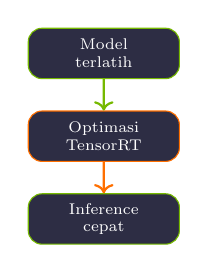
\begin{tikzpicture}[scale=0.8, every node/.style={transform shape},
          b/.style={draw=nvgreen, fill=nvcard, rounded corners=5pt, text=white, font=\scriptsize, minimum width=2.4cm, minimum height=0.8cm, align=center}]
        \node[b] (m) {Model\\terlatih};
        \node[b, below=0.5cm of m, draw=nvorange] (o) {Optimasi\\TensorRT};
        \node[b, below=0.5cm of o, draw=nvgreen] (i) {Inference\\cepat};
        \draw[->,thick,color=nvgreen] (m)--(o);
        \draw[->,thick,color=nvorange] (o)--(i);
      \end{tikzpicture}
      \end{center}
    \end{column}
  \end{columns}
  \vspace{0.2em}
  \begin{beamercolorbox}[rounded=true,shadow=false,sep=4pt]{block body}
    \centering\small\color{white}
    Di Module 06 TensorRT hanya \textbf{di-install} \& dibahas konseptual --- tidak ada demo (notebook memakai PyTorch).
  \end{beamercolorbox}
\end{frame}

% ── Act 2: NVIDIA NeMo ────────────────────────────────────
\acttitle{2}{NVIDIA NeMo}{Toolkit untuk Conversational AI}

% Slide 7 — Apa itu NeMo
\begin{frame}{Apa itu NeMo?}
  \framesubtitle{Toolkit conversational AI dari NVIDIA}
  \begin{itemize}
    \item \textbf{NeMo} (Neural Modules): toolkit \textbf{open-source} NVIDIA untuk \textbf{conversational AI} (AI percakapan)
    \item Cakupan: pemahaman teks, terjemahan, sampai sintesis suara
    \item Kaya \textbf{pre-trained model} (siap pakai) --- tak perlu melatih dari nol
    \item Modular: komponen dirangkai bebas seperti balok lego
    \item Skalabel karena dioptimalkan untuk \textbf{GPU} NVIDIA
  \end{itemize}
  \vspace{0.5em}
  \begin{beamercolorbox}[rounded=true,shadow=false,sep=6pt]{block body}
    \centering\small\color{nvlightgreen}
    Inti NeMo: unduh model AI canggih, panggil method-nya, langsung pakai --- tanpa training dari awal.
  \end{beamercolorbox}
\end{frame}

% Slide 8 — Peta Tugas NeMo
\begin{frame}{Peta Tugas NeMo}
  \framesubtitle{6 task conversational AI yang didemokan}
  \begin{center}
    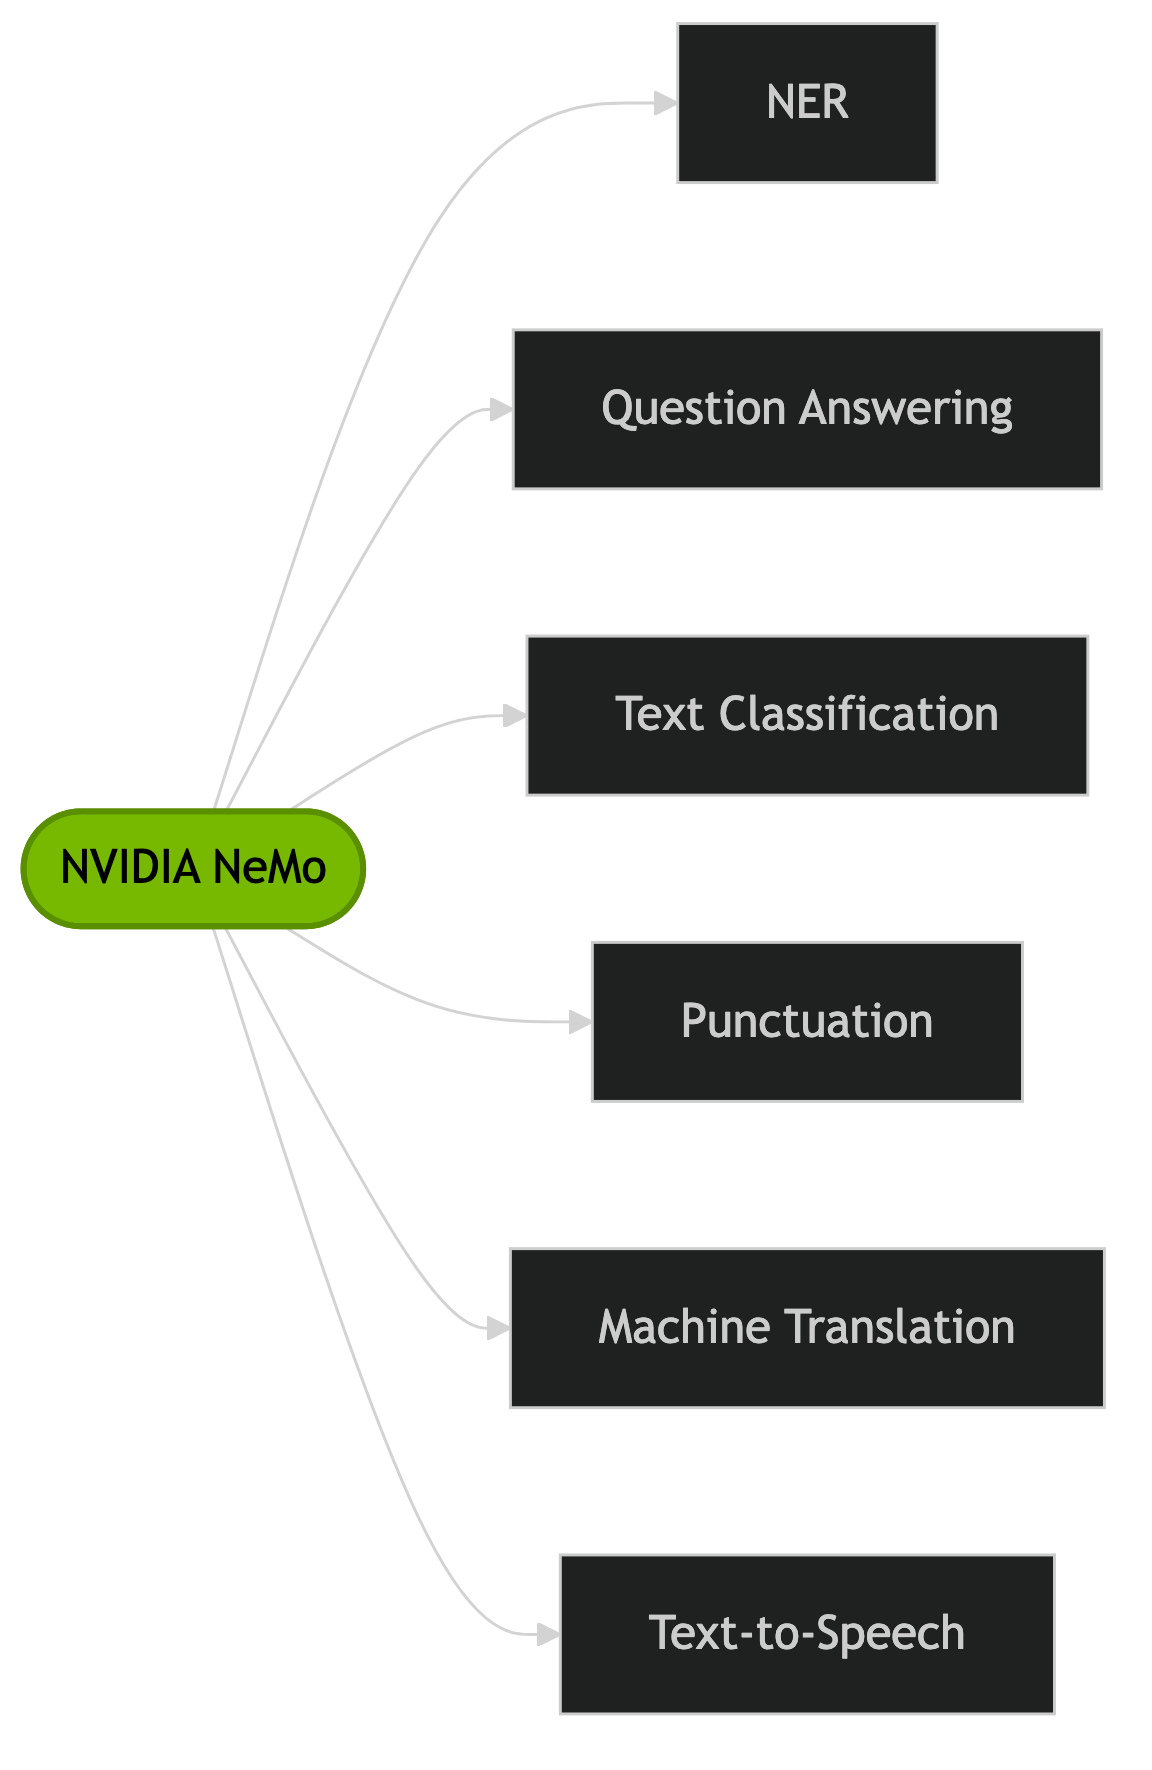
\includegraphics[height=0.6\textheight]{figures/nemo_tasks.png}
  \end{center}
  \vspace{0.2em}
  \begin{center}\textcolor{nvlightgreen}{\small Satu toolkit, enam task --- semuanya cukup dengan \textbf{pre-trained model} siap pakai.}\end{center}
\end{frame}

% Slide 9 — NER & QA
\begin{frame}[fragile]{NER \& Question Answering}
  \framesubtitle{Memahami dan menjawab dari teks}
  \begin{columns}[T]
    \begin{column}{0.52\textwidth}
      \begin{itemize}
        \footnotesize
        \item \textbf{NER}: \texttt{TokenClassificationModel} + \texttt{ner\_en\_bert} (berbasis \textbf{BERT})
        \item \texttt{add\_predictions()} menandai entitas: "NVIDIA" $\to$ ORG, "New York" $\to$ LOC
        \item \textbf{QA}: \texttt{QAModel} + \texttt{qa\_squadv1.1\_bertbase}
        \item Model prediksi posisi \texttt{start} \& \texttt{end} jawaban di konteks
      \end{itemize}
    \end{column}
    \begin{column}{0.46\textwidth}
      \begin{lstlisting}[language=Python, basicstyle=\ttfamily\scriptsize\color{nvwhite}]
model = TokenClassificationModel \
    .from_pretrained("ner_en_bert")
results = model.add_predictions(texts)
      \end{lstlisting}
    \end{column}
  \end{columns}
  \vspace{0.2em}
  \begin{center}\textcolor{nvlightgreen}{\small NER menandai SIAPA/DI MANA; QA menunjuk potongan teks (start--end) yang menjawab pertanyaan.}\end{center}
\end{frame}

% Slide 10 — Text Classification & Punctuation
\begin{frame}[fragile]{Text Classification \& Punctuation}
  \framesubtitle{Mengelompokkan dan merapikan teks}
  \begin{columns}[T]
    \begin{column}{0.52\textwidth}
      \begin{itemize}
        \footnotesize
        \item \textbf{Text Classification}: \texttt{TextClassificationModel} $\to$ kategori (mis. sentimen)
        \item \texttt{classifying()} memberi label per kalimat
        \item \textbf{Punctuation}: \texttt{PunctuationCapitalizationModel} + \texttt{punctuation\_en\_bert}
        \item Contoh: "nvidia is a company" $\to$ "Nvidia is a company."
      \end{itemize}
    \end{column}
    \begin{column}{0.46\textwidth}
      \begin{lstlisting}[language=Python, basicstyle=\ttfamily\scriptsize\color{nvwhite}]
text = "nvidia is a company"
model.add_punctuation_capitalization(
    [text])[0]
      \end{lstlisting}
    \end{column}
  \end{columns}
  \vspace{0.2em}
  \begin{center}\textcolor{nvlightgreen}{\small Klasifikasi memberi label; punctuation mengubah teks polos jadi rapi (berguna untuk hasil transkripsi).}\end{center}
\end{frame}

% Slide 11 — MT & TTS
\begin{frame}[fragile]{Machine Translation \& TTS}
  \framesubtitle{Lintas bahasa dan teks ke suara}
  \begin{columns}[T]
    \begin{column}{0.5\textwidth}
      \begin{itemize}
        \footnotesize
        \item \textbf{MT}: \texttt{MTEncDecModel} + \texttt{nmt\_en\_zh\_transformer24x6} (Inggris $\to$ Mandarin)
        \item \texttt{translate()} terima daftar kalimat
        \item \textbf{TTS}: pipeline 2 tahap berurutan
        \item Tahap 1 \texttt{FastPitch}: teks $\to$ \textbf{spectrogram}
        \item Tahap 2 \texttt{HiFiGAN} (\textbf{vocoder}): spectrogram $\to$ audio
      \end{itemize}
    \end{column}
    \begin{column}{0.48\textwidth}
      \begin{lstlisting}[language=Python, basicstyle=\ttfamily\tiny\color{nvwhite}]
parsed = spec_gen.parse(text)
spec = spec_gen.generate_spectrogram(
    tokens=parsed)
audio = vocoder \
    .convert_spectrogram_to_audio(spec=spec)
      \end{lstlisting}
    \end{column}
  \end{columns}
  \vspace{0.2em}
  \begin{center}\textcolor{nvlightgreen}{\small TTS $=$ 2 tahap: teks jadi spectrogram (FastPitch), lalu spectrogram jadi audio (HiFiGAN).}\end{center}
\end{frame}

% Slide 12 — Catatan Penting
\begin{frame}{Catatan Penting}
  \framesubtitle{Sebelum menjalankan demo NeMo}
  \begin{itemize}
    \item[\textcolor{nvorange}{$\bullet$}] Demo ini \textbf{berat di GPU} --- jangan dijalankan semua sekaligus
    \item[\textcolor{nvgreen}{\checkmark}] Sifatnya \textbf{konseptual}: fokus memahami ALUR tiap task
    \item[\textcolor{nvorange}{$\bullet$}] Notebook meng-import model \textbf{ASR} (speech recognition) \& \texttt{MegatronGPTModel}\ldots
    \item[\textcolor{nvorange}{$\bullet$}] \ldots tetapi keduanya \textbf{TIDAK didemonstrasikan} --- import $\neq$ dipakai
    \item[\textcolor{nvgreen}{\checkmark}] Lihat \textbf{Module 02} (dasar GPU) \& \textbf{Module 05} (dasar RAG)
  \end{itemize}
  \vspace{0.4em}
  \begin{beamercolorbox}[rounded=true,shadow=false,sep=6pt]{block body}
    \centering\small\color{white}
    Baca kode dengan teliti: meng-\textbf{import} model (ASR \& Megatron) tidak sama dengan men-\textbf{demokan}-nya.
  \end{beamercolorbox}
\end{frame}

% ── Act 3: NVIDIA-Accelerated RAG ─────────────────────────
\acttitle{3}{NVIDIA-Accelerated RAG}{RAG dipercepat GPU}

% Slide 13 — RAG di atas Stack NVIDIA
\begin{frame}{RAG di atas Stack NVIDIA}
  \framesubtitle{Menjalankan RAG dengan akselerasi GPU}
  \begin{itemize}
    \footnotesize
    \item \textbf{RAG} (\textbf{Retrieval-Augmented Generation}) $=$ pencarian dokumen $+$ \textbf{LLM} agar jawaban berbasis fakta (dasar di \textbf{Module 05})
    \item Fokus di sini: sudut \textbf{tooling NVIDIA} --- \textbf{embedding} \& LLM dipindah ke \textbf{GPU} (\texttt{.to('cuda')})
    \item Install \textbf{faiss-gpu} bersama \texttt{nemo\_toolkit}, \texttt{transformers}
  \end{itemize}
  \vspace{0.4em}
  \begin{center}
  
\begin{tikzpicture}[scale=0.9, every node/.style={transform shape},
      b/.style={draw=nvgreen, fill=nvcard, rounded corners=4pt, text=white, font=\scriptsize, minimum width=1.7cm, minimum height=0.7cm, align=center}]
    \node[b] (d) {Dokumen};
    \node[b, right=0.5cm of d] (e) {Embedding\\\tiny(GPU)};
    \node[b, right=0.5cm of e] (f) {FAISS};
    \node[b, right=0.5cm of f] (l) {LLM gpt2\\\tiny(GPU)};
    \node[b, right=0.5cm of l, draw=nvorange] (a) {Jawaban};
    \draw[->,thick,color=nvgreen] (d)--(e); \draw[->,thick,color=nvgreen] (e)--(f);
    \draw[->,thick,color=nvgreen] (f)--(l); \draw[->,thick,color=nvorange] (l)--(a);
  \end{tikzpicture}
  \end{center}
\end{frame}

% Slide 14 — Arsitektur NvidiaRAGSystem
\begin{frame}[fragile]{Arsitektur NvidiaRAGSystem}
  \framesubtitle{Empat komponen dalam satu pipeline}
  \begin{columns}[T]
    \begin{column}{0.46\textwidth}
      \begin{itemize}
        \footnotesize
        \item \textbf{Embedding}: SentenceTransformer (\texttt{all-MiniLM-L6-v2}) di GPU
        \item \textbf{Index}: \textbf{FAISS} (\texttt{IndexFlatL2})
        \item \textbf{Generator}: LLM \textbf{gpt2} di GPU
        \item \textbf{Doc}: \textbf{cudf} (RAPIDS) bungkus dokumen $\to$ pandas
      \end{itemize}
    \end{column}
    \begin{column}{0.54\textwidth}
      \begin{lstlisting}[language=Python, basicstyle=\ttfamily\tiny\color{nvwhite}]
self.embedding_model = SentenceTransformer(
    'all-MiniLM-L6-v2').to(self.device)
self.llm = AutoModelForCausalLM \
    .from_pretrained("gpt2").to(self.device)
df = cudf.DataFrame(
    {'text': documents}).to_pandas()
      \end{lstlisting}
    \end{column}
  \end{columns}
  \vspace{0.1em}
  \begin{center}\textcolor{nvlightgreen}{\small \texttt{cudf} hanya membungkus dokumen lalu langsung \texttt{.to\_pandas()} (chunking pakai Python biasa).}\end{center}
\end{frame}

% Slide 15 — Module 05 vs 06
\begin{frame}{Module 05 vs Module 06: Tooling NVIDIA}
  \framesubtitle{RAG yang sama, tooling berbeda}
  \begin{center}
  \renewcommand{\arraystretch}{1.3}
  {\scriptsize
  \setlength{\tabcolsep}{4pt}
  \begin{tabular}{@{}p{0.24\linewidth}p{0.36\linewidth}p{0.32\linewidth}@{}}
    \toprule
    \rowcolor{nvcard!50}
    \textbf{Aspek} & \textbf{Module 05 (RAG dasar)} & \textbf{Module 06 (NVIDIA)} \\
    \midrule
    Penempatan model & \texttt{device\_map="auto"}, float32 & GPU eksplisit (\texttt{.to(cuda)}) \\
    Embedding & all-MiniLM-L6-v2 & all-MiniLM-L6-v2 \\
    LLM & TinyLlama (float32) & gpt2 \\
    FAISS & faiss-cpu & faiss-gpu (install) \\
    Doc handling & Python biasa & cudf (RAPIDS) $\to$ pandas \\
    \bottomrule
  \end{tabular}%
  }
  \end{center}
  \vspace{0.3em}
  \begin{center}\textcolor{nvlightgreen}{\small Pipeline RAG tetap sama; yang ditukar adalah \textbf{tooling}-nya.}\end{center}
\end{frame}

% Slide 16 — Alur Demo & Catatan
\begin{frame}{Alur Demo \& Catatan}
  \framesubtitle{demonstrate\_rag(): retrieve $\to$ augment $\to$ generate}
  \begin{itemize}
    \footnotesize
    \item \textbf{Retrieve}: \texttt{retrieve\_relevant\_chunks()} cari potongan termirip via FAISS (\texttt{k=3})
    \item \textbf{Augment}: gabung query $+$ konteks jadi satu \textbf{prompt}
    \item \textbf{Generate}: \texttt{generate\_response()} pakai gpt2 menulis jawaban
  \end{itemize}
  \vspace{0.4em}
  \begin{beamercolorbox}[rounded=true,shadow=false,sep=6pt]{block body}
    \small\color{white}
    \textcolor{nvorange}{\textbf{Catatan akurasi:}} \texttt{MegatronGPTModel} hanya di-\emph{import}; LLM yang dipakai $=$ \textbf{gpt2}. \texttt{faiss-gpu} di-install, tapi \texttt{IndexFlatL2} sebenarnya dibangun di \textbf{CPU}.
  \end{beamercolorbox}
\end{frame}

% Slide 17 — Ringkasan & Akhir Course
\begin{frame}{Ringkasan \& Akhir Course}
  \framesubtitle{Ekosistem NVIDIA menutup perjalanan kita}
  \begin{columns}[T]
    \begin{column}{0.5\textwidth}
      \textcolor{nvgreen}{\textbf{Module 06:}}
      \begin{itemize}
        \footnotesize
        \item \textbf{GPU/CUDA}: fondasi akselerasi
        \item \textbf{NeMo}: toolkit conversational AI siap pakai
        \item \textbf{RAG} dipercepat: faiss-gpu, model di GPU
      \end{itemize}
    \end{column}
    \begin{column}{0.48\textwidth}
      \textcolor{nvlightgreen}{\textbf{Perjalanan course:}}
      \begin{itemize}
        \footnotesize
        \item[\textcolor{nvgreen}{\checkmark}] 01 Machine Learning
        \item[\textcolor{nvgreen}{\checkmark}] 02 Deep Learning
        \item[\textcolor{nvgreen}{\checkmark}] 03 NLP \quad 04 LLM
        \item[\textcolor{nvgreen}{\checkmark}] 05 RAG \quad 06 NVIDIA
      \end{itemize}
    \end{column}
  \end{columns}
  \vspace{0.4em}
  \begin{beamercolorbox}[rounded=true,shadow=false,sep=6pt]{block body}
    \centering\small\color{white}
    Dari \textbf{machine learning} klasik hingga \textbf{LLM} \& \textbf{RAG} yang dipercepat GPU --- pondasi lengkap untuk membangun AI modern.
  \end{beamercolorbox}
\end{frame}

% Slide 18 — Thank You
\begin{frame}[plain]
  \vspace{2cm}
  \begin{center}
    {\color{nvgreen}\Huge\bfseries Terima Kasih!}\\[1.2em]
    {\color{nvwhite}\Large Selamat --- Anda telah menyelesaikan seluruh course!}\\[1.5em]
    \begin{beamercolorbox}[rounded=true,shadow=false,sep=8pt,wd=10cm]{block body}
      \centering\color{white}
      \textbf{NVIDIA Ecosystem} \quad $\cdot$ \quad Modul 06 \\
      Navasena Gen-ML Course
    \end{beamercolorbox}
  \end{center}
\end{frame}

\end{document}
